\teteSndAP
\vspace*{-36pt}
\titreActivite*{La biodiversité}

\begin{multicols}{2}

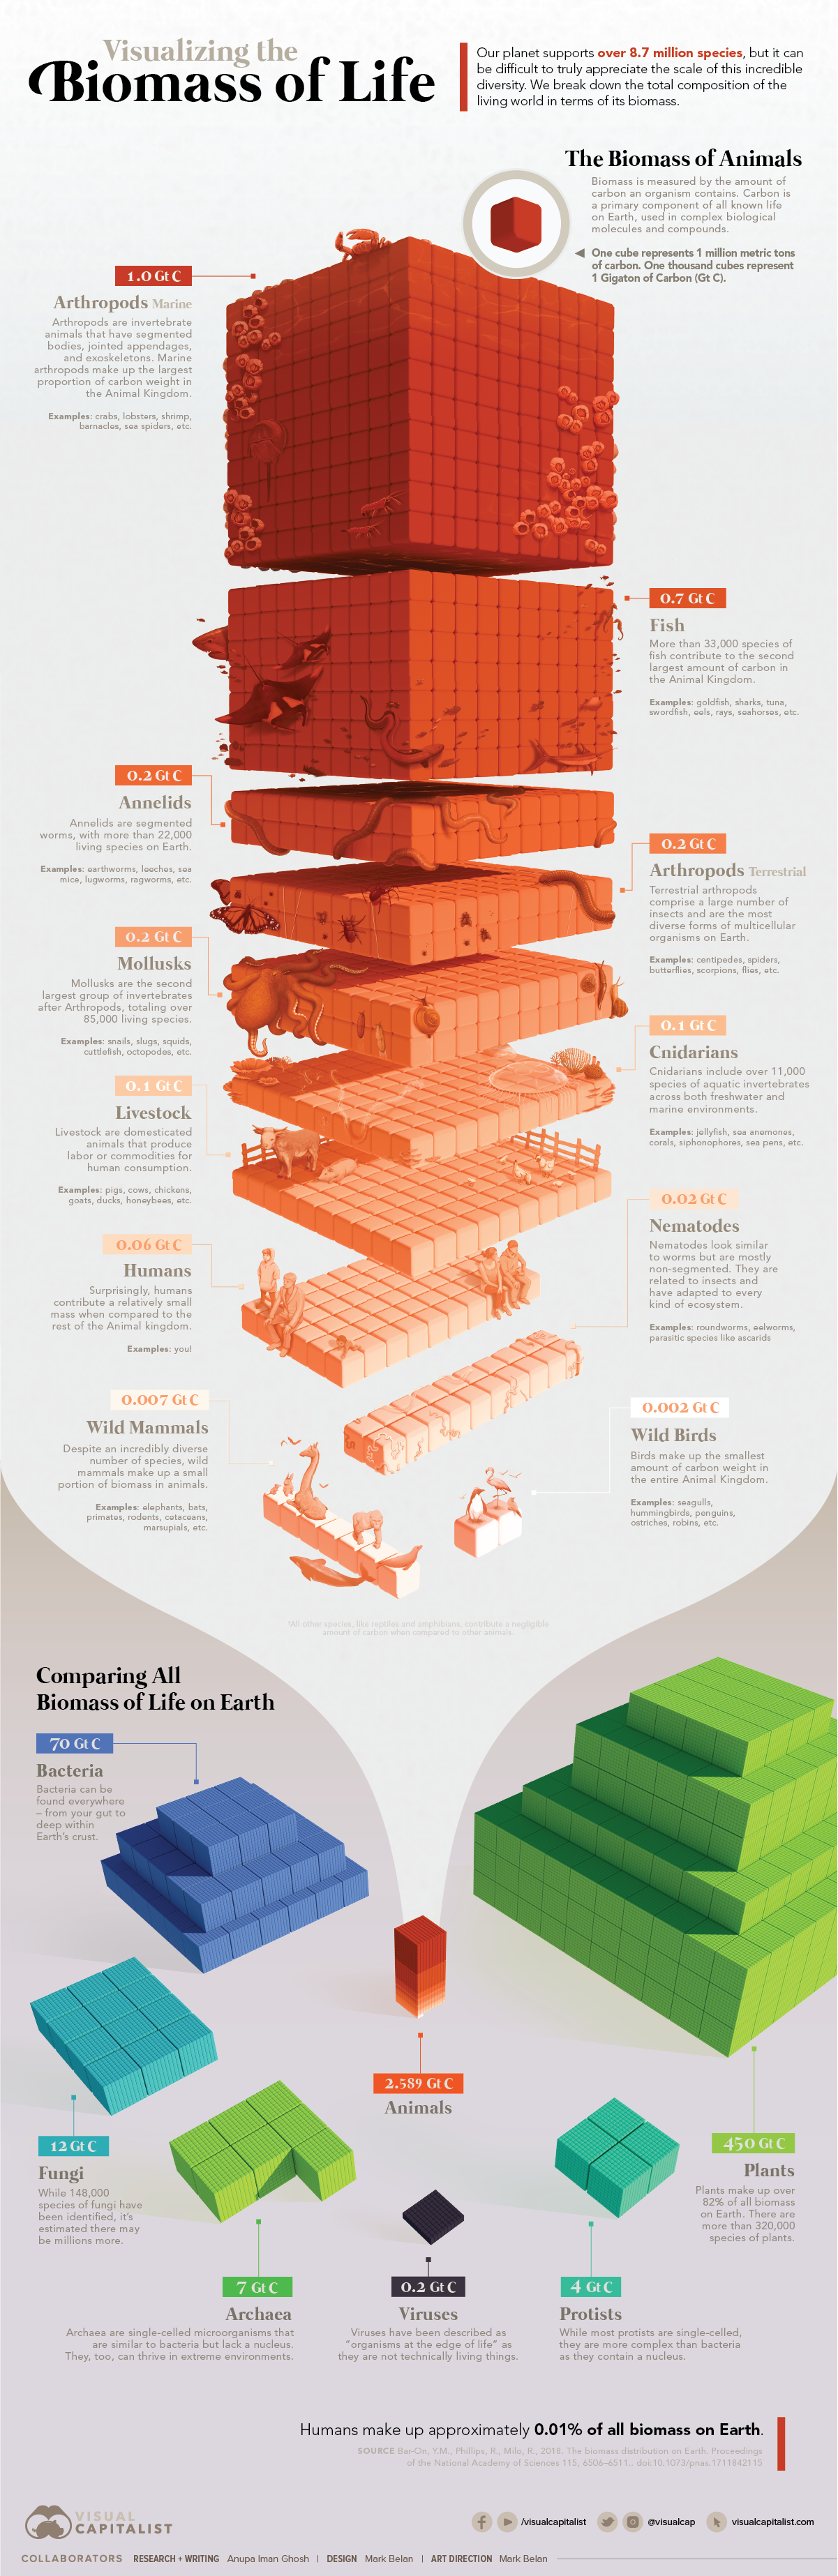
\includegraphics[height=\textheight]{accompagnement_personnel/Visualizing-the-biomass-of-earth}

\begin{objectifs}
  \item Comprendre les trois échelles de biodiversité : écosystèmes, espèces, individus.
  \item Revoir la théorie de l'évolution.
\end{objectifs}

\begin{contexte}
  La « \important{biodiversité} » désigne la diversité du vivant sous toutes ses formes, du microscopique au macroscopique.
  
  \problematique{
    Comment quantifier la biodiversité dans le monde et autour de nous ? 
    Quels activités humaines menacent la biodiversité ?
  }
\end{contexte}
\begin{doc}{Trois rang de biodiversité}{doc:A_echelle_biodiversite}
  La \important{biodiversité} est la diversité des êtres vivants sur Terre. 
  La biodiversité peut être décrite à trois échelles différentes :
  \begin{listePoints}
    \item La diversité des \important{écosystèmes} regroupe la diversité des organismes vivant dans un lieu précis et les interactions existant entre les différents organismes.
    \item La diversité des \important{espèces} au sein d'un écosystème.
    \item La diversité des \important{individus} au sein d'une même espèce.
  \end{listePoints}

  Pour étudier la biodiversité, il faut donc recenser toutes les espèces qui vivent dans un lieu et étudier les populations de chaque espèces, c'est pourquoi la recherche participative est souvent utilisée, à travers des journées de mobilisation ou des applications.
\end{doc}

\begin{doc}{Quelques ordres de grandeur sur la biomasse}{doc:A_odg_biomasse}
  \textcolor{couleurPrim}{\faArrowLeft} Visualisation des ordres de grandeurs pour la biomasse sur Terre.

  On retiendra que la majorité de la biomasse est constitué d'être vivants microscopiques et de plantes.
  Même parmi les animaux, les humains et les animaux domestiques ou d'élevages représentent une faible fraction de la biomasse.
  
  Dans une forêt, il y a plus de diversité sous terre qu'en dehors !
\end{doc}

\end{multicols}

\begin{doc}{La théorie de l'évolution}{doc:A_theorie_evolution}
  \qrcodeCote{https://www.youtube.com/watch?v=GhHOjC4oxh8}
  
  Pour expliquer l'incroyable diversité du vivant actuel, on utilise \important{la théorie de l'évolution}.

  \begin{listePoints}
    \item \important{sélection naturelle}
    \item \important{dérive génétique}
    \item \important{la spéciation}
  \end{listePoints}
\end{doc}

% - 1 séance pour faire un état des lieux sur c'est quoi la biodiversité ?
%   - les trois échelles : écosystèmes (forêt urbaine lol), espèces, individus
%   - rappel de quelques ordres de grandeurs sur la biomasse 
%   - la théorie de l'évolution -> https://www.youtube.com/watch?v=lIEoO5KdPvg
%   - sortie plant.net et bird.net 
  
% - 1 séance sur une sous thématique :
%   - biodiversité passé
%   - biodiversité actuelle
%   - préservation / renforcement de la biodiversité
%     - aménagement urbains, préservation/renforcement en milieu urbain
%     - accueillir la biodiversité chez soi
%   - évolution de la biodiversité
  
% - visite au muséum d'histoire naturelle : 
%   - 8h30 rdv au blanc
%   - 3h au jardin 
%     - 1 h galerie évolution
%     - 1 h galerie d'anatomie comparée
%     - 1 h dans le parc en commun -> parc botanique
%   - arrivée au blanc à 14h